%!TEX root = P231_notes.tex

\section{The Harmonic Oscillator}
% \lecdate{lec~12}

Let's return to the problem of solving for Green's functions. Let's focus on our favorite example---arguably, the \emph{only} example\footnote{Upon generalizing to higher dimensions, curvilinear coordinates. Physicists have Harmonic Oscillators in different area codes.}---is the harmonic oscillator. The differential operator is
\begin{align}
	\mathcal O = \left(\frac{d}{dt}\right)^2 + \omega_0^2 \ .
	\label{eq:O:HO}
\end{align}
The Green's function equation tells us the response $G(t,t_0)$ at time $t$ from a `unit displacement' at $t_0$:
\begin{align}
	G''(t,t_0) + \omega_0^2 G(t,t_0) = \delta(t-t_0) \ .
	\label{eq:HO:Greens:eqn}
\end{align}
Recall that the arguments $t$ and $t_0$ are analogous to the indices of a finite-dimensional matrix. For notational convenience, we will set $t_0=0$ and not list it explicitly. We are primarily concerned about the $t$-dependence of $G(t,t_0)$. 

\subsection{Fourier Transform}

The first thing we're going to do is write $G(t,t_0)$ as a Fourier transform with respect to $t$. Please refer to Appendix~\ref{app:Fourier} for our set of Fourier transform conventions. We can write $G(t)$ as an integral over Fourier modes with frequency $\omega$ and weight (Fourier transform) $\tilde G(\omega)$:
\begin{align}
	G(t) &= \int_{-\infty}^\infty\dbar \omega \, e^{-i\omega t} \tilde G(\omega) 
	&
	\dbar = \frac{d}{2\pi}
	\ .
	\label{eq:HO:Greens:Fourier}
\end{align}
We say that $\tilde G(\omega)$ is the Fourier transform of $G(t)$. The key point is that the $t$-dependence of $G(t)$ has been sequestered into the $e^{-i\omega t}$ plane waves. This is convenient since these plane waves are eigenfunctions of the derivative operator:
\begin{align}
	\frac{d}{dt} e^{-i\omega t} &= -i\omega e^{-i\omega t} \ .
\end{align}
The left-hand side of the Green's function equation \eqref{eq:HO:Greens:eqn} is
\begin{align}
	\mathcal O_t G(t,t_0) 
	&= 
	-
	\int_{-\infty}^\infty \dbar \omega \, 
	\left(\omega^2-\omega_0^2\right) e^{-i\omega t} \tilde G(\omega,t_0) \ .
\end{align}
The right-hand side is simply the Fourier transform of $\delta(t-t_0)$:
\begin{align}
	\delta(t-t_0)
	&=
	\int_{-\infty}^\infty \dbar \omega \, e^{-i\omega (t-t_0)} \ .
	\label{eq:delta:fourier}
\end{align}
\begin{exercise}
Use our conventions for the Fourier transform \eqref{eq:HO:Greens:Fourier} (see also Appendix~\ref{app:Fourier}) to confirm the Fourier representation of $\delta(t-t_0)$ in \eqref{eq:delta:fourier}. In our notation, the Fourier coefficients $\tilde f(\omega)$ of a function $f(t)$ is
\begin{align}
	\tilde f(\omega) &= 
	% \frac{1}{2\pi}
	\int_{-\infty}^\infty d t\, e^{i\omega t} f(t) \ .
\end{align}
\end{exercise}
So the Green's function equation for the 1D harmonic oscillator, \eqref{eq:HO:Greens:eqn}, tells us
\begin{align}
	-
	\int_{-\infty}^\infty \dbar \omega \, 
	\left(\omega^2-\omega_0^2\right) e^{-i\omega t} \tilde G(\omega)
	&=
	\int_{-\infty}^\infty \dbar \omega \, e^{i\omega t}
	\ .
	\label{eq:G:HO:Fourier:equation:integrals}
\end{align}
For simplicity we have set $t_0=0$ and don't write it explicitly. There's a rather unscrupulous\footnote{I don't think this is rigorously valid, but the result is true. The ends don't justify the means, but let's take this morally ambiguous shortcut to make the big picture clear. I encourage you to live the rest of your lives with virtue.} way to solve this equation for $\tilde G(\omega)$. Since the two sides of this expression are equal, they have the same Fourier expansion. This implies that the Fourier coefficients are equal. Since both sides are already written as Fourier expansions, we can just match the coefficients of the basis functions, $e^{-i\omega t}$. This gives us:
\begin{align}
	\tilde G(\omega) &= \frac{-1}{\omega^2-\omega_0^2}
	\label{eq:G:HO:Fourier:term}
\end{align}
\begin{exercise}
Prove \eqref{eq:G:HO:Fourier:term} honestly. {Hint}: Start with \eqref{eq:G:HO:Fourier:equation:integrals} and project out the Fourier coefficients. Recall that you do this by taking the inner product with one of the basis functions and then using the orthogonality of the eigenbasis. You may need to be careful with the normalization.
\end{exercise}
\begin{exercise}
In \eqref{eq:G:HO:Fourier:equation:integrals} we had already set $t_0 = 0$. What is the expression for $\tilde G(\omega)$ if we kept $t_0$ explicit?
\label{eq:ex:Gtilde:with:t0:explicit}
\end{exercise}
That was the critical step: we have successfully solved for the Green's function Fourier coefficient. This means that we have a closed form expression for the Green's function by plugging $\tilde G(\omega)$ into \eqref{eq:HO:Greens:Fourier}:
\begin{align}
	G(t) &=  \int_{-\infty}^\infty \dbar \omega
	\, 
	\frac{-e^{-i\omega t}}{\omega^2-\omega_0^2} \ .
	\label{eq:G:HO:Fourier:Rep:t0:0}
\end{align}
All that's left is for us to actually \emph{do} this integral. Fortunately, this integral should look very similar. It seems to beg for us to solve using the residue theorem. 
\begin{exercise}
What are the poles of the integrand in \eqref{eq:G:HO:Fourier:Rep:t0:0}? What are their associated residues? What is the residue if $t_0\neq 0$?
\end{exercise}

\subsection{Contour Integral}

The integral \eqref{eq:G:HO:Fourier:Rep:t0:0} looks like it's perfect for contour integration. There's an exponential factor on top that will determine the convergence, and the denominator can be factored to see where the poles are. Except we notice something troubling:
\begin{align}
	\frac{-e^{-i\omega t}}{\omega^2-\omega_0^2} 
	&=
	\frac{-e^{-i\omega t}}{(\omega - \omega_0)(\omega + \omega_0)} \ .
	\label{eq:HO:integrand:real:pole}
\end{align}
The poles are located at $\omega = \pm \omega_0$. These are \emph{on the real axis}, precisely along the integration contour! How annoying!

Now you may want to have an existential moment. Remind yourself that all we're doing is solving for the behavior of the one-dimensional \emph{harmonic oscillator}. This is an eminently \emph{physical} system. We could have written this system as $\mathcal O f(t) = s(t)$ where $f(t)$ is the displacement of a harmonic oscillator and $s(t)$ is some driving function. The Green's function, $G(t,t_0)$ gives the response of the system to a `unit' driving function, $s(t) = \delta(t-t_0)$. The response of the system should be perfectly physical. And yet---\emph{and yet}---we now face an integral \eqref{eq:G:HO:Fourier:Rep:t0:0} that seems to run right into not only one, but \emph{two} singularities along the integration contour!
\begin{center}
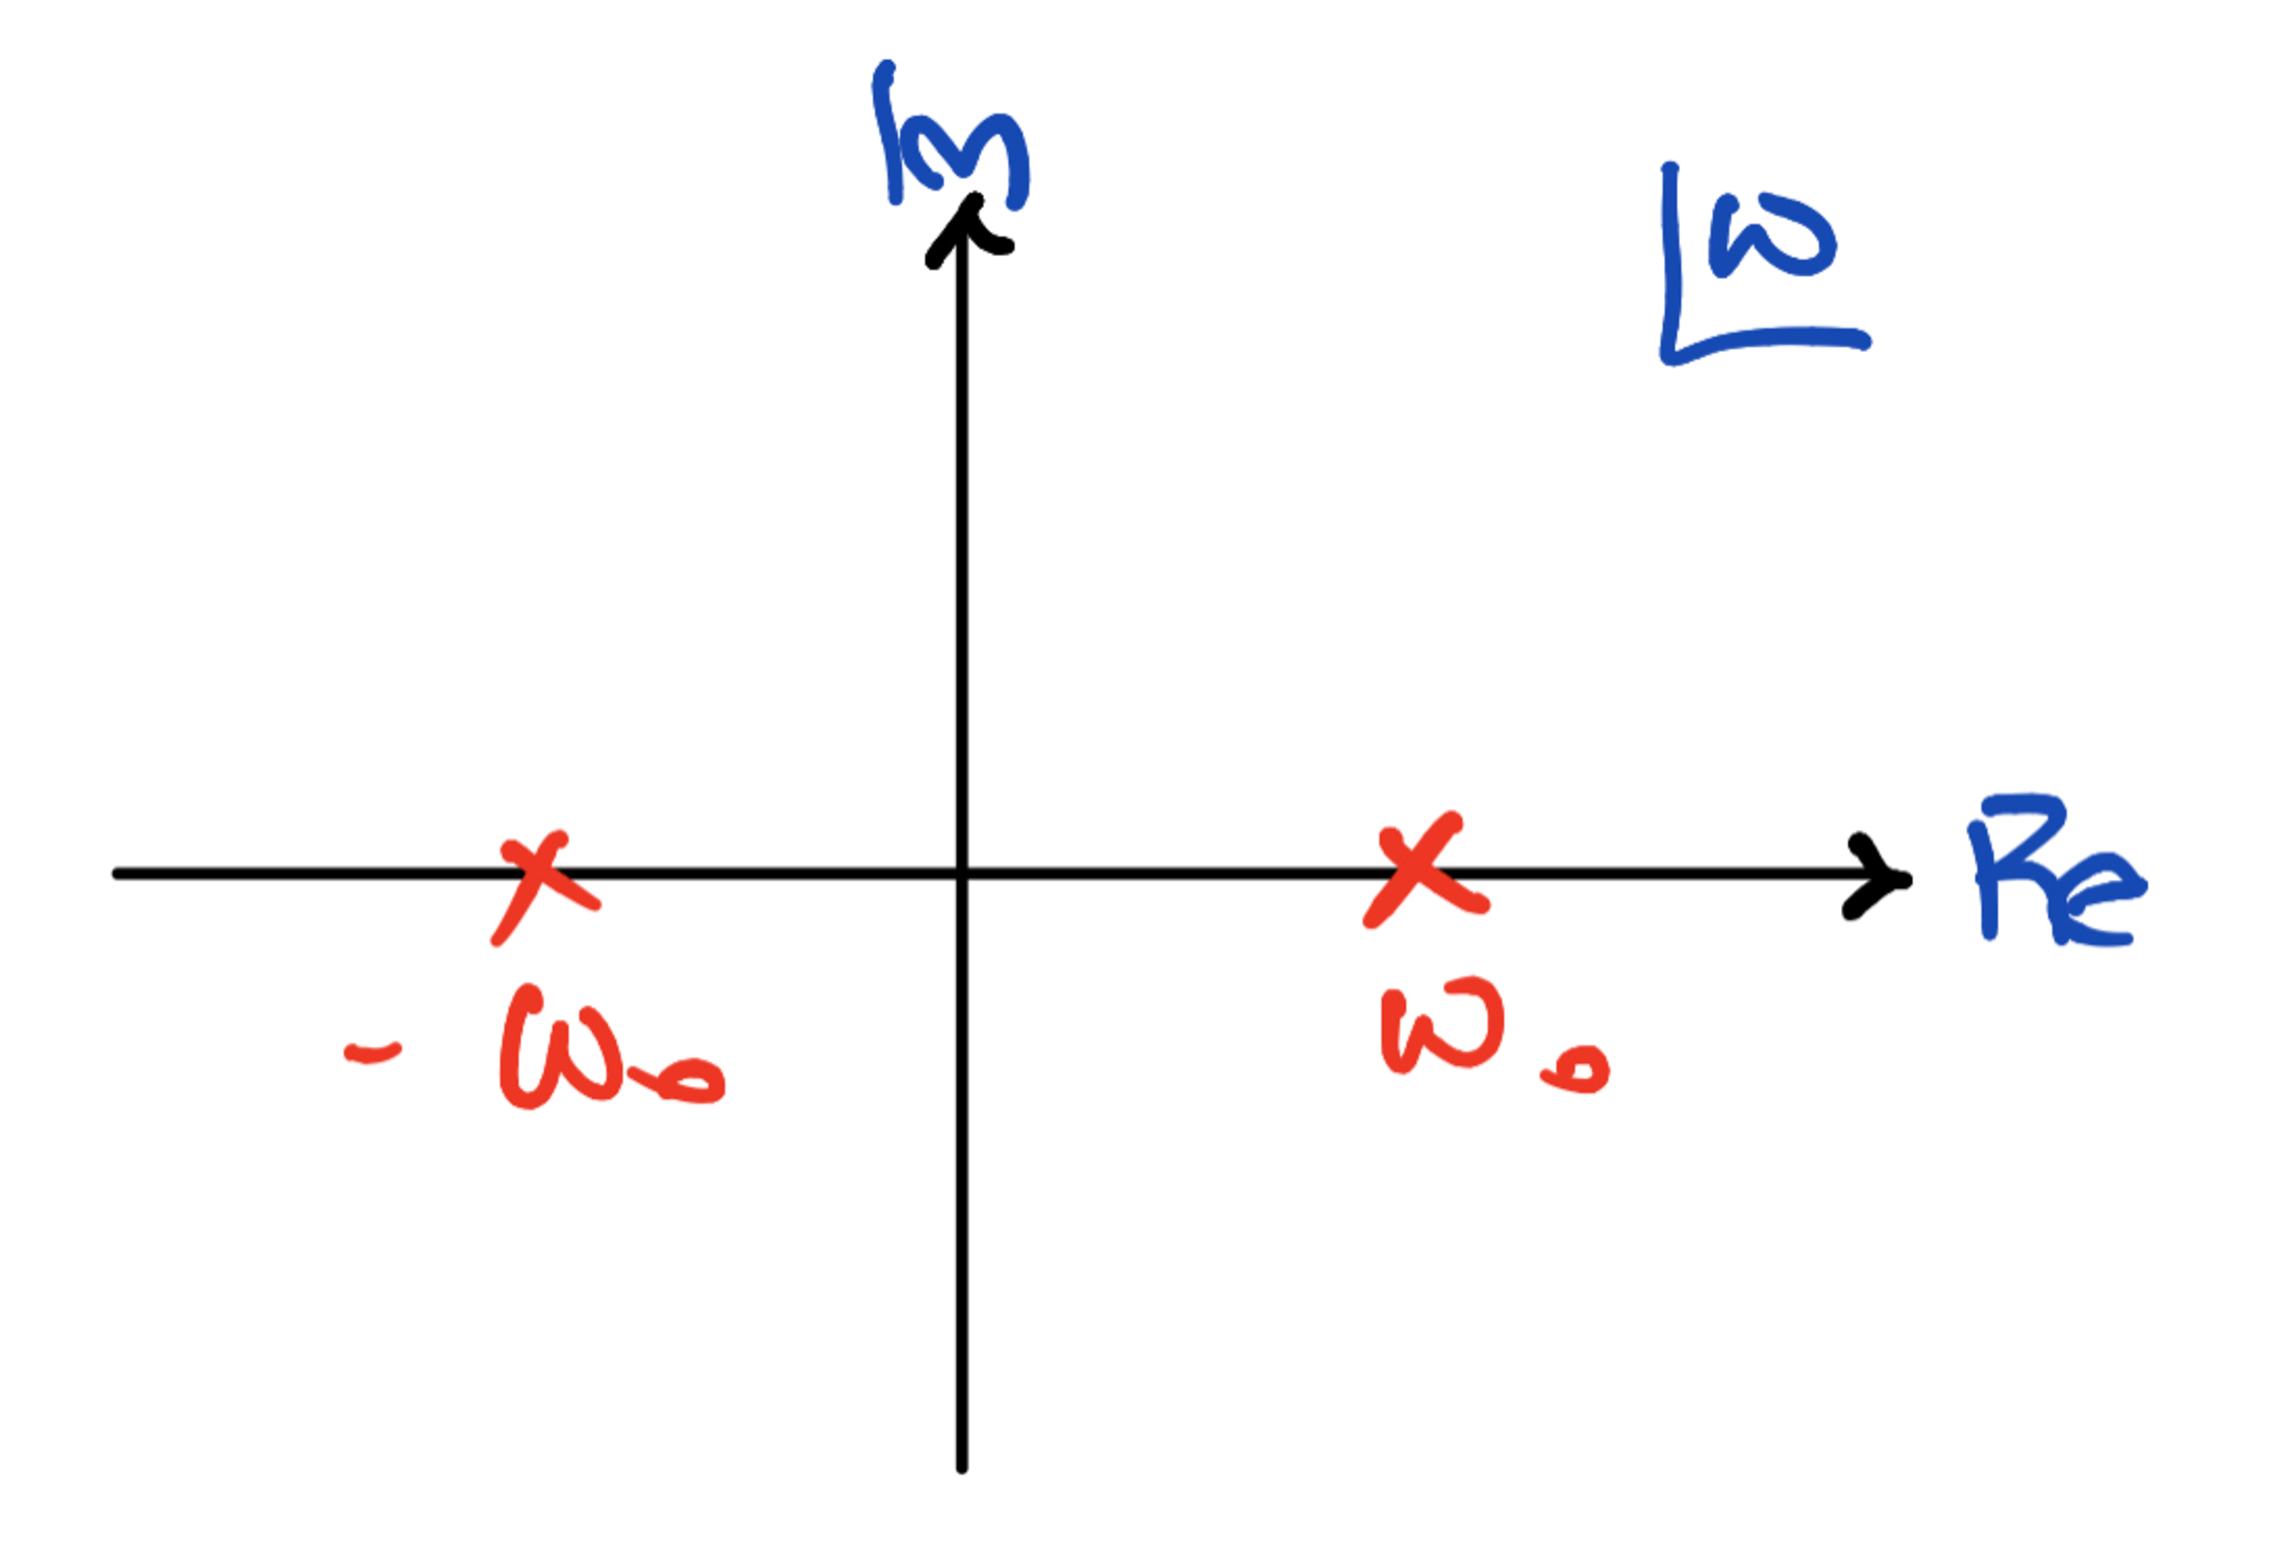
\includegraphics[width=.4\textwidth]{figures/Lec_2017_16_HO_Poles.pdf}
\end{center}
Please do take a brief moment to ponder at this existential crisis. This is an apparent failure of our theory---our calculation hits a pole, you get an infinity, and it's not clear what's going on. Rather than anguish, though, we should see if our theory is trying to tell us something. 

In order to figure out what's going on, let's do something wild. The poles on the real axis are in the way. Let's just move them out of the way by giving them small imaginary parts\footnote{I have altered the poles. Pray that I do not alter them further.}. Each pole can either be pushed above or below the real line:
\begin{center}
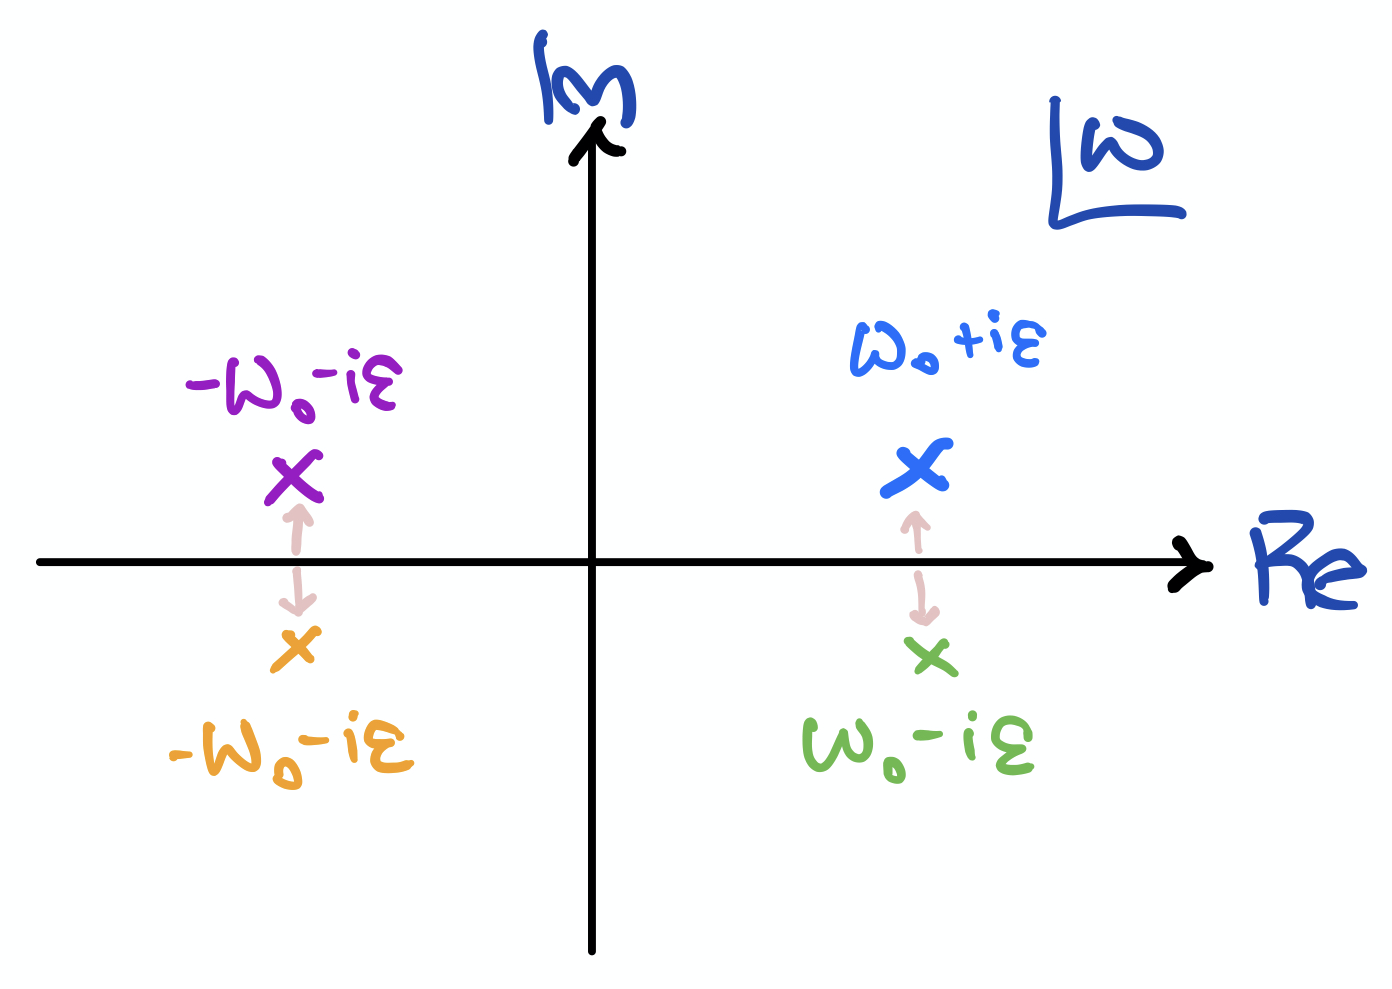
\includegraphics[width=.4\textwidth]{figures/Lec_2017_16_HO_PoleShift.png}
\end{center}
To be clear: are \emph{changing} the integral. We are exploring what happens when the expression \eqref{eq:G:HO:Fourier:Rep:t0:0} is changed, as if the poles were slightly complex the whole time. In other words, we are \emph{changing} the original differential operator, \eqref{eq:O:HO}. We're not yet motivating \emph{why} we want to do this; we'll justify it post-facto. For now, let's just be happy that our contours no longer bump into the poles. 

\subsection{Going under the poles?}
Let's try going under the poles, that is: let's push the poles into the upper half-plane with small imaginary parts:
\begin{center}
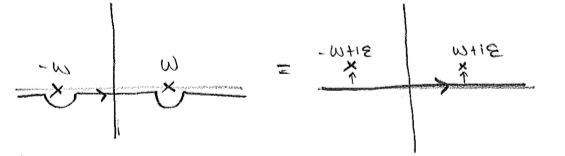
\includegraphics[width=.6\textwidth]{figures/Lec_2017_16_underpole.png}
\end{center}
This means that we have deformed the integrand \eqref{eq:HO:integrand:real:pole}:
\begin{align}
\frac{-e^{-i\omega t}}{(\omega - \omega_0)(\omega + \omega_0)}
&\to
\frac{-e^{-i\omega t}}{(\omega - \omega_0 - i\varepsilon)(\omega + \omega_0 - i\varepsilon)} \ .
\label{eq:HO:integrand:upper:poles}
\end{align}
To make it clear that we are treating $\omega$ as a complexified variable, let's write it as $z$:
\begin{align}
 	\omega \to z \ .
 \end{align}
Now let's go through the exercise of performing the integral along the real line by using the residue theorem. To do this have to choose a contour that includes the real line. We have two options, $C_+$ and $\bar C_-$, where the bar reminds us of the orientation:
\begin{center}
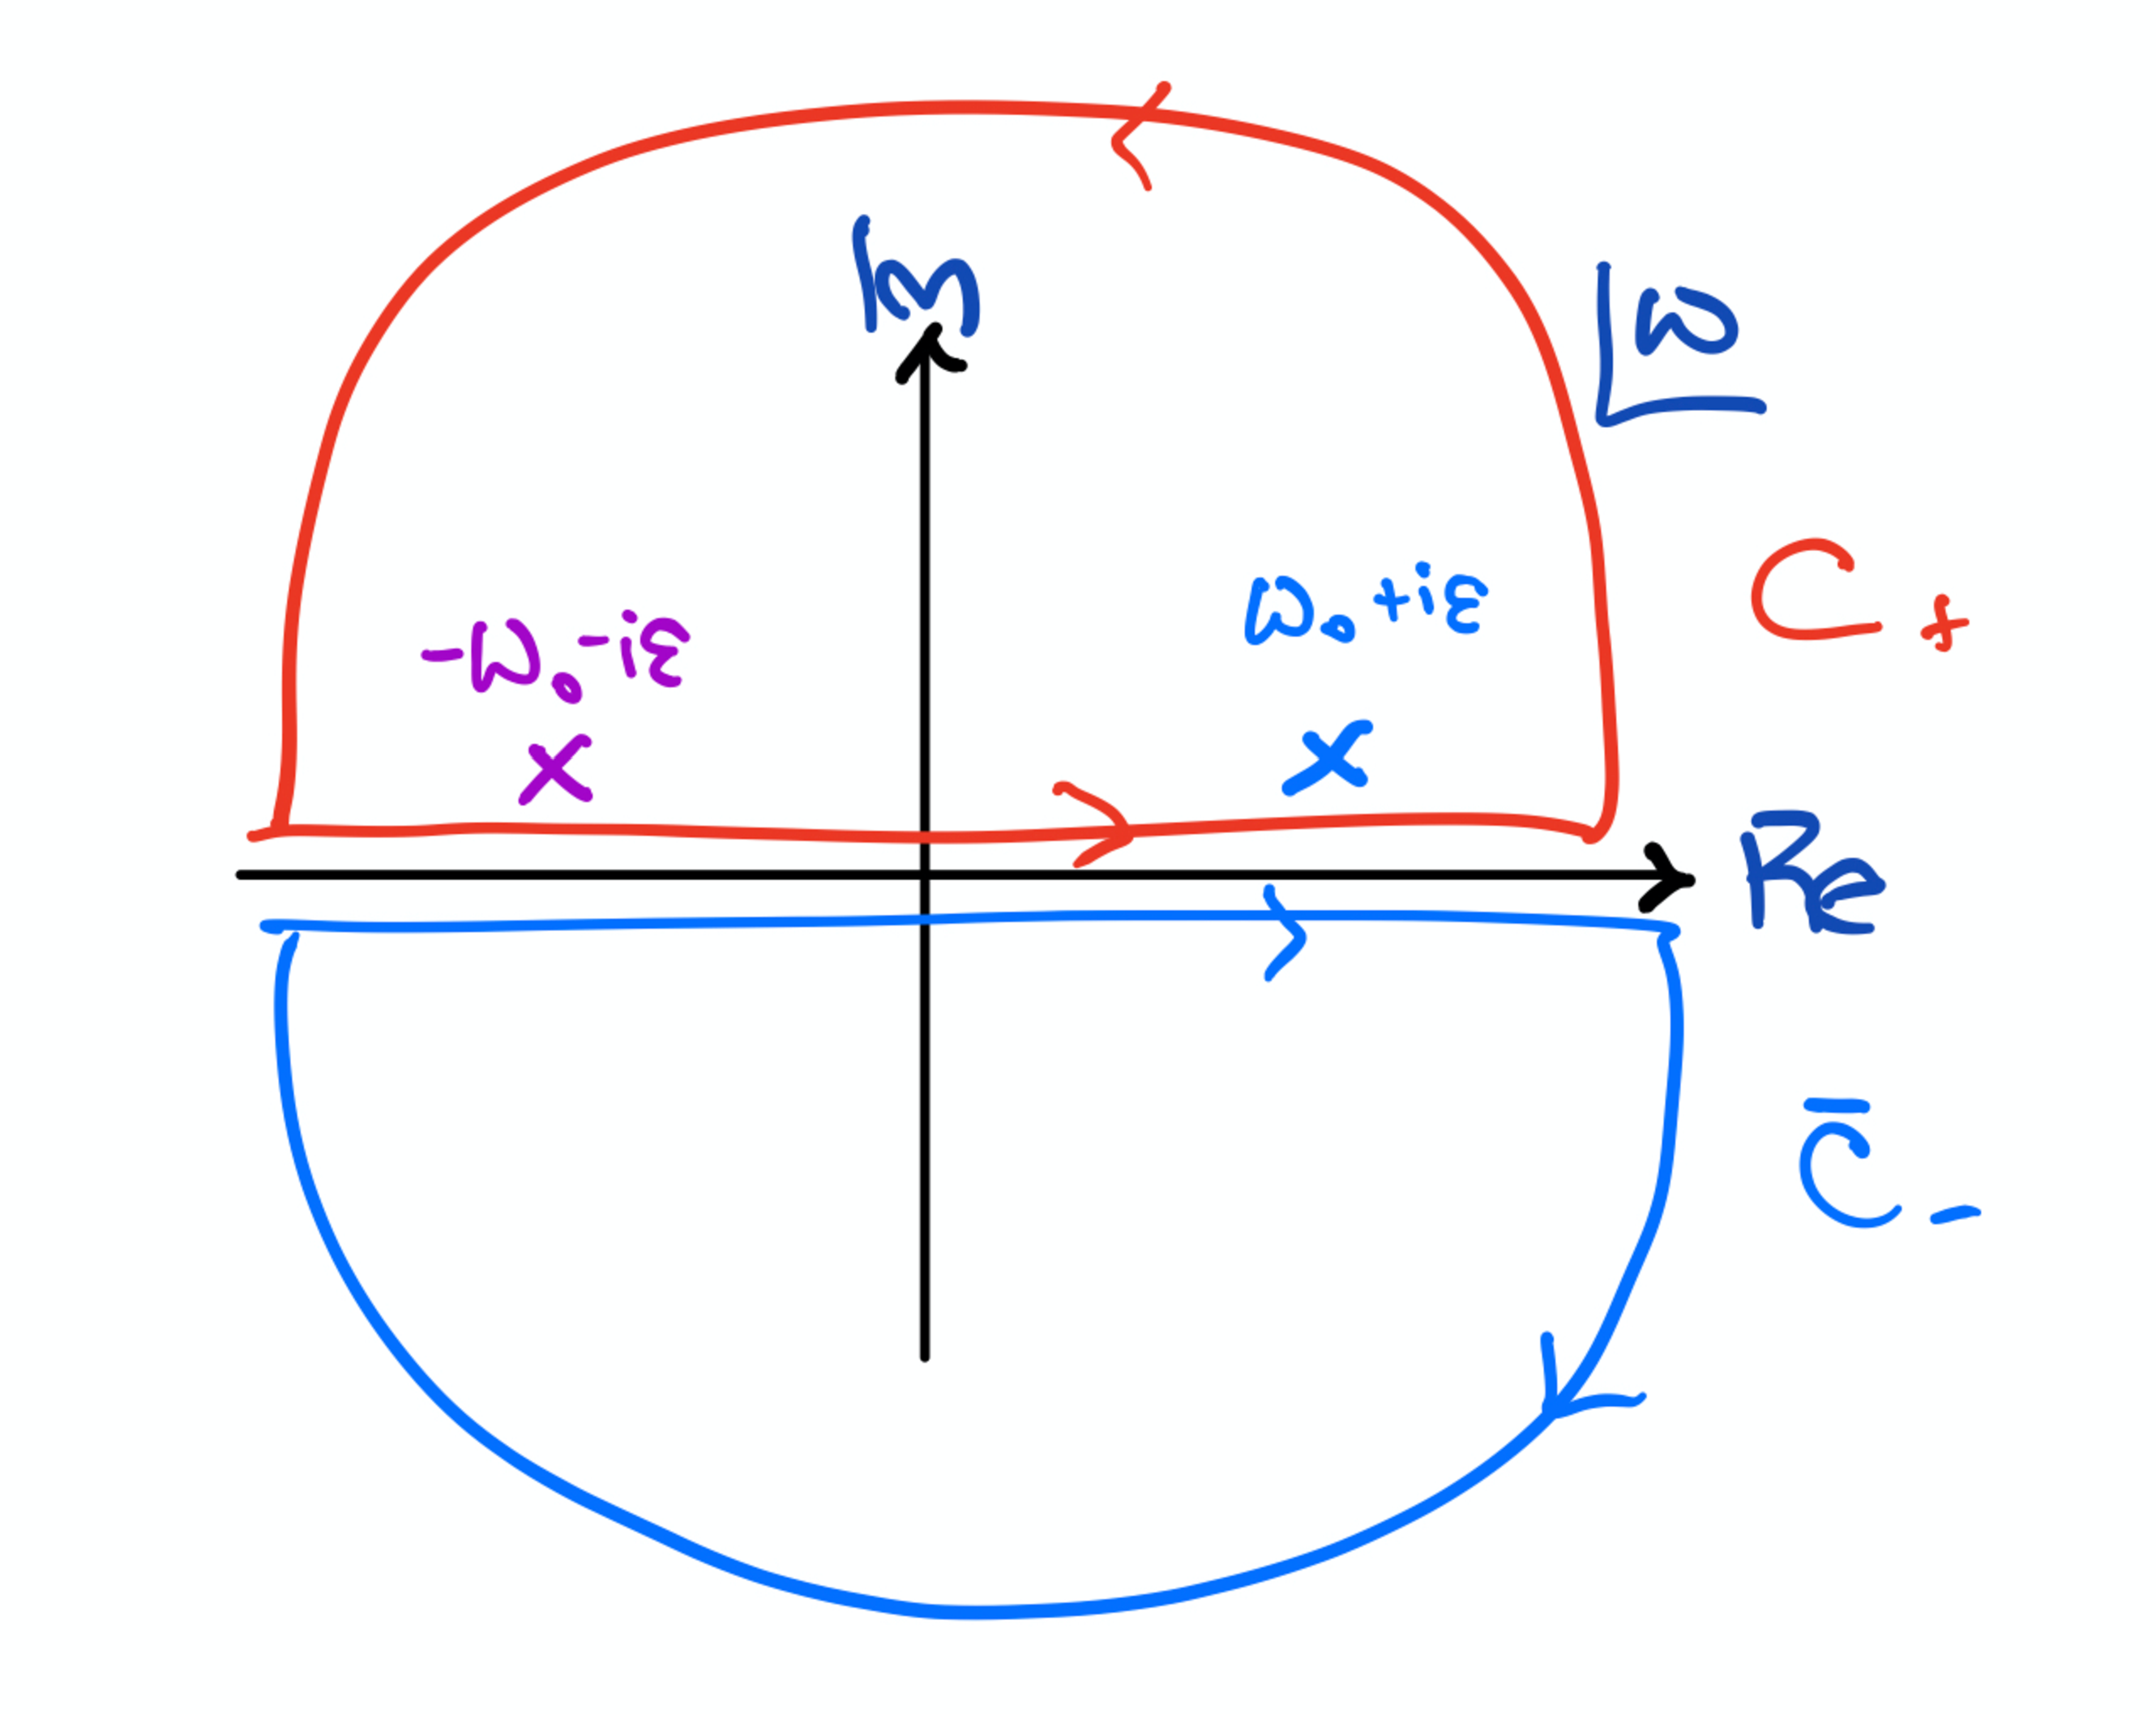
\includegraphics[width=.4\textwidth]{figures/Lec_2017_16_pokeup.pdf}
\end{center}
Which contour do we pick? Does it matter? (Yes!) The contours differ by whether the `large arc' has positive or negative real part. We can parameterize these arcs as we did in \eqref{eq:z:paramterization:large:arc}:
\begin{align}
	z(\theta) &= R\cos\theta + i R\sin\theta \ ,
\end{align}
where for $C_+$ the arc is given by $\theta \in [0,\pi]$ while for $\bar C_-$ the arc is $\theta\in[\pi,2\pi]$. In other words, 
\begin{align}
	\text{for $C_+$:}\, \sin\theta &> 0
	&
	\text{for $\bar C_-$:}\, \sin\theta &<0 \ .
	\label{eq:HO:which:contour}
\end{align}
%
How do we pick? The criteria for completing the real line into a contour is that the integral along the contour vanishes, that way
\begin{align}
	\oint_C dz\, f(z) 
	= \int_{-\infty}^\infty dx\, f(x) + \lim_{R\to \infty} R \int_\text{arc} d\theta f(Re^{i\theta}) 
	= \int_{-\infty}^\infty dx\, f(x) \ .
\end{align}
And hence one can use the residue theorem to solve the contour integral on the left-hand side and relate it to the real integral on the right-hand side\footnote{I say `real integral' but of course the integrand \eqref{eq:HO:integrand:upper:poles} is now a complex quantity, but the point is that we're only integrating along the real line.}. 
%
So which contour satisfies
\begin{align}
	\lim_{R\to \infty} R \int_\text{arc} d\theta 
	% f(Re^{i\theta})  
	\frac{-e^{-i(R\cos\theta + iR\sin\theta) t}}{(Re^{i\theta} - \omega_0 - i\varepsilon)(Re^{i\theta} + \omega_0 - i\varepsilon)}
	\to 0 \ ?
\end{align}
I was a little slick and chose to write $z = R\cos\theta + iR\sin\theta$ in the numerator while writing the more compact $z=Re^{i\theta}$ in the denominator. The convergence\footnote{I tend to say convergence, what I really mean is `vanishes as $R\to \infty$.'} of the integrand depends on the exponential factor in the numerator:
\begin{align}
	e^{-i(R\cos\theta + iR\sin\theta) t} = 
	e^{-iRt\cos\theta} e^{Rt\sin\theta} \ .
\end{align}
We can see that the convergence depends specifically on the second factor, $e^{-Rt\sin\theta}$. Since $R>0$, this depends on two things: the sign of $\sin\theta$ and the sign of $t$. The integral along the arc vanishes in the $R\to\infty$ limit when:
\begin{align}
	t > 0 \quad\text{and}\quad \sin\theta < 0 &
	&\text{or}&&
	t < 0 \quad\text{and}\quad \sin\theta > 0 \ .
	\label{eq:t:gtr:less:upper:poles}
\end{align}
Or in other words:
\begin{align}
	t>0 &\to \bar C_{-} 
	&
	t<0 &\to C_+ \ .
	\label{eq:t:sign:contour:HO}
\end{align}
% \begin{itemize}
% 	\item $t>0$ and $\sin\theta > 0$ or
% 	\item $t<0$ and $\sin\theta < 0$ \ .
% \end{itemize}
Recall that we have set $t_0 = 0$; if you did Exercise~\ref{eq:ex:Gtilde:with:t0:explicit}, you would know that restoring $t_0$ corresponds to $t\to t-t_0$ in the conditions above.

The Green's function equation \eqref{eq:Greens:func:as:inverse} is simply that $$\mathcal O_t G(t,t') = \delta(t-t')\ .$$ This tells us that the Green's function $G(t,t')$ is the \emph{response} measured at time $t$ to a $\delta$-function source at $t_0$. Thus the sign of $t-t_0$ corresponds to whether we are measuring the response \emph{before} or \emph{after} the cause. If you are like me, your eyes just lit up with joy. Something very exciting has happened: in this odd discussion about pushing around the poles of $\tilde G$, we have found that we were secretly talking about \emph{causality}.  

Before we progress, let's be clear: we expect that effects happen \emph{after} causes. This means that physical dynamics obey $t-t_0 >0$. A nice theory would tell us that you cannot have an effect before a cause\footnote{At the beginning of this course, we talked about locality as one of the motivating factors for why physical dynamics are described by differential operators. This was closely tied to the idea of causality, since non-local effects with spacelike separation can be non-causal in some reference frame. Perhaps amusingly---but beyond the scope of this course or my expertise---the notion of causality and locality in fundamental theories of nature continues to be a theme in cutting edge theoretical research.}. 

\paragraph{Causal propagation.}
For the specific case of $t>0$ (or $t-t_0>0$ if we restore $t_0$), we observe from \eqref{eq:t:gtr:less:upper:poles} that the integral \eqref{eq:HO:integrand:upper:poles} converges when $\sin\theta <0$. In other words, for times \emph{after} the initial cause at $t_0=0$, the appropriate contour is $\bar C_-$. 
\begin{exercise}
What is the value of the contour integral 
\begin{align}
	\oint_{\bar{C}_-} dz\, \frac{-e^{-i z t}}{(z - \omega_0 - i\varepsilon)(z + \omega_0 - i\varepsilon)} \ ?
\end{align}
Hint: you shouldn't have to do any work.
\end{exercise}
The contour integral above vanishes along the arc when $t>0$, so it is the correct contour when doing the Fourier transform to get $G(t)$ from $\tilde G(\omega)$. However, the contour encloses no poles. No poles means no residues. This means that the contour integral vanishes and the Fourier transform vanishes. In other words, 
\begin{align}
	G(t>0) &= 0 \ .
	\label{eq:HO:G:t:gtr:0:zero}
\end{align}

\begin{example}
The statement that $G(t>0)=0$ should make you sad and possibly upset. This means that there is \emph{no} effect that happens after some cause at $t_0=0$.
\end{example}

\paragraph{Acausal propagation.} By now you see the writing on the wall. Something perverse has happened: after a $\delta$-function disturbance, information is not traveling forward in time because $G(t)=0$ for $t>0$. This, in turn, was self-evident in because for $t>0$, we were required to take the $\bar C_-$ contour in order that the contribution of the arc vanishes. At this point, you must feel the dread of what's coming next. If we take the $t<0$ case in \eqref{eq:t:gtr:less:upper:poles}, we are forced to take the $C_+$ contour. This contour indeed picks up poles and so we expect it to be non-zero. Thus we find that $G(t<0) \neq 0$, which is awful because this $t<0$ corresponds to an \emph{effect that happens before the cause}. 

\begin{exercise}
Taking $t_0=0$ for simplicity, show that the exact result for the acausal Green's function is
\begin{align}
	G(t<0) &= \frac{-1}{\omega_0}\sin\omega_0t \ .
	\label{eq:HO:G:t:less:0:nonzero}
\end{align}
Hint: the relevant residues are $\pm e^{\pm i\omega_0t}/2\omega_0$ \ .
\end{exercise}
You should \emph{do} the above exercise as practice for the main contour integral of this entire course. If you are tempted to just keep reading these notes\footnote{By now you should know that learning physics requires \emph{doing} physics. Reading/watching someone else do physics is one of the least efficient ways of improving yourself as a physicist.} 

To help you along, let me even set up the integral for you. We start with $G(t)$ in \eqref{eq:HO:integrand:real:pole}, where we rewrote the integrand in \eqref{eq:G:HO:Fourier:Rep:t0:0} to make the pole structure clear. We then said that we wanted to push the poles off the real line. This \emph{changes} the physical problem, but we'll worry about what that means later. In this case, we move the poles into the upper half-plane so that each pole has a small imaginary part. The poles are then located at $\pm \omega_0 + i \varepsilon$. The resulting integral is:
\begin{align}
	G(t) &= 
	\int_{-\infty}^\infty \frac{d\omega}{2\pi} 
	\frac{-e^{-i\omega t}}{(\omega - \omega_0-i\varepsilon)(\omega + \omega_0-i\varepsilon)} 
	\ .
\end{align}
Complete the real integral into a contour integral; we'll re-label our variables to remind us that we're in the complex plane, $\omega\to z$. The contour that we select, $C_+$, came from the $e^{-i\omega t}$ factor. The result is:
\begin{align}
	\oint_{C_+}
	\frac{dz}{2\pi} 
	\frac{-e^{-iz t}}{(z - \omega_0-i\varepsilon)(z + \omega_0-i\varepsilon)}
	=&\phantom{+} 
	\int_{-\infty}^\infty \frac{d\omega}{2\pi} 
	\frac{-e^{-i\omega t}}{(\omega - \omega_0-i\varepsilon)(\omega + \omega_0-i\varepsilon)} 
	\nonumber
	\\
	&
	+ 
	\cancel{
	\lim_{R\to\infty} \int_{0}^\pi \frac{Rd\theta}{2\pi} 
	\frac{-e^{-i(R\cos\theta + i R\sin\theta)t}}{(Re^{i\theta} - \omega_0-i\varepsilon)(Re^{i\theta} + \omega_0-i\varepsilon)} 
	}
	\label{eq:HO:G:integral:adv:1}
	\\
	&=
	2\pi i \sum_{z_\pm=\pm\omega_0+i\varepsilon} \text{Res}_f(z) \ ,
	\label{eq:HO:G:integral:adv:2}
\end{align}
where $f$ is understood to be the integrand. 
%
From here you should be able to read off the result. Confirm that we can take the $\varepsilon\to 0$ limit; this tiny shift was only there to tell us that the poles live in the upper half-plane.

\paragraph{Advanced propagator.}
The causal ($t>0$) and acausal ($t<0$) cases in \eqref{eq:HO:G:t:less:0:nonzero} and \eqref{eq:HO:G:t:gtr:0:zero} respectively may be combined into a single expression:
\begin{align}
	G_\text{adv}(t) &= \frac{-1}{\omega_0}\sin(\omega_0t) \Theta(-t) \ ,
	\label{eq:HO:G:adv:theta}
\end{align}
where we use the Heaviside step function
\begin{align}
	\Theta(x) = 
	\begin{cases}
	1 & \text{if}\; x>0\\
	0 & \text{if}\; x<0 \ .
	\end{cases}
	\label{eq:Heaviside:Theta}
\end{align}
This is the \textbf{advanced} propagator. Even though `advanced' is often a positive adjective when applied to your progress\footnote{I once read a story about a particle physicist who started a conversation with a stranger on the plane. The stranger explains, ``My son is really quite brilliant. He's studying physics at an Ivy league university.'' The physicist says, ``Oh, how nice. You know, I'm a physicist.''  The stranger then asks what kind of physics, to which the physicist says ``I study elementary particles.'' The stranger responds with, ``Ah yes. Well, my son studies advanced particles.'' I no longer remember where I read this story, but I can attest to meeting people like this.} In this context, however, `advanced' is a \emph{bad} word. It means \emph{acausal}: the cause comes \emph{after} the effect. This does not make any sense, and we reject this as non-sense. 

After an appropriate amount of indignant disdain, we can reflect on how the heck we got here\footnote{If your response is \emph{Christmas! Christmas eve last year}, then I applaud your taste in musical theater.}. We make two observations:
\begin{enumerate}
\item After checking all of our work, the main conclusion from this non-sense result is that our approach of pushing the poles \emph{up} into the upper half-plane must have been wrong. We see that the position of the poles tells us about the causality of the system. By pushing the poles off the real axis, we have imposed a sense of causality in time. We should see what happens when we push the poles \emph{down} into the lower half-plane. 

\item Even though the \emph{physics} of advanced propagator is utter rubbish because it breaks causality, we also appreciate that it is a perfectly reasonable \emph{mathematical} solution. The harmonic oscillator dynamics encoded in our differential operator $\mathcal O_t$ is symmetric with respect to time-reversal symmetry\footnote{The behavior of our models under $t\to -t$ is a powerful diagnostic for understanding our physical theories. One of my friends was in a pub the night before lecture and some of the pub regulars, who knew he was a physicists, asked him what he was lecturing on the next day. He said he was going to talk about reversing the direction of time, to which they cautiously responded: `\emph{... we can do that??}'}. The `physical' interpretation is analogous to seeing a bunch of ripples starting at the edges of a pond that move inward until they reach a singularity ($\delta$-function!?) at which point the pond spits out a small pebble. 
\end{enumerate}


\begin{exercise}
At this point, you should be able to solve the case of the causal Green's function without any additional guidance. In fact, without doing any work, you should see that by pushing the poles down into the lower half plane, the propagator will be causal. With a little bit of thought, you may be able to write the analog of \eqref{eq:HO:G:adv:theta}, the retarded Green's function\footnote{In the same way that `advanced' means something different colloquially versus for physics, we use this word very carefully. One of my friends in graduate school was an international student who liked to make physics puns. At some point she playfully admonished late arriving undergraduates for being `retarded,' which required quite a bit of care to clarify the situation to everyone involved.}, without doing any work. You should still proceed to calculate $G_\text{ret}(t)$ the `honest way.' We walk  through it together in the next subsection. 
\label{ex:retarded:G:HO}
\end{exercise}


\subsection{Going over the poles}

Assuming that you have completed Exercise~\ref{ex:retarded:G:HO}, you have figured out the main result of this course\footnote{Do the exercises. I've come to appreciate how annoying it is to come up with meaningful exercises, rather than rote calculations. At some point there's a phase transition in education where exercises are no longer just `practice' but are pedagogical tools to make sure your brain knows how to \emph{think} physics rather than just \emph{read} physics. To say it differently, as my undergraduate advisor once told me: you should do every single exercise problem you can. If you're short on time, just focus on the ones that you cannot do.}. However, because this example is so important, let's go ahead and walk through it together. We push the poles down into the lower half-plane by giving them a small imaginary part, $-i\varepsilon$.

\begin{center}
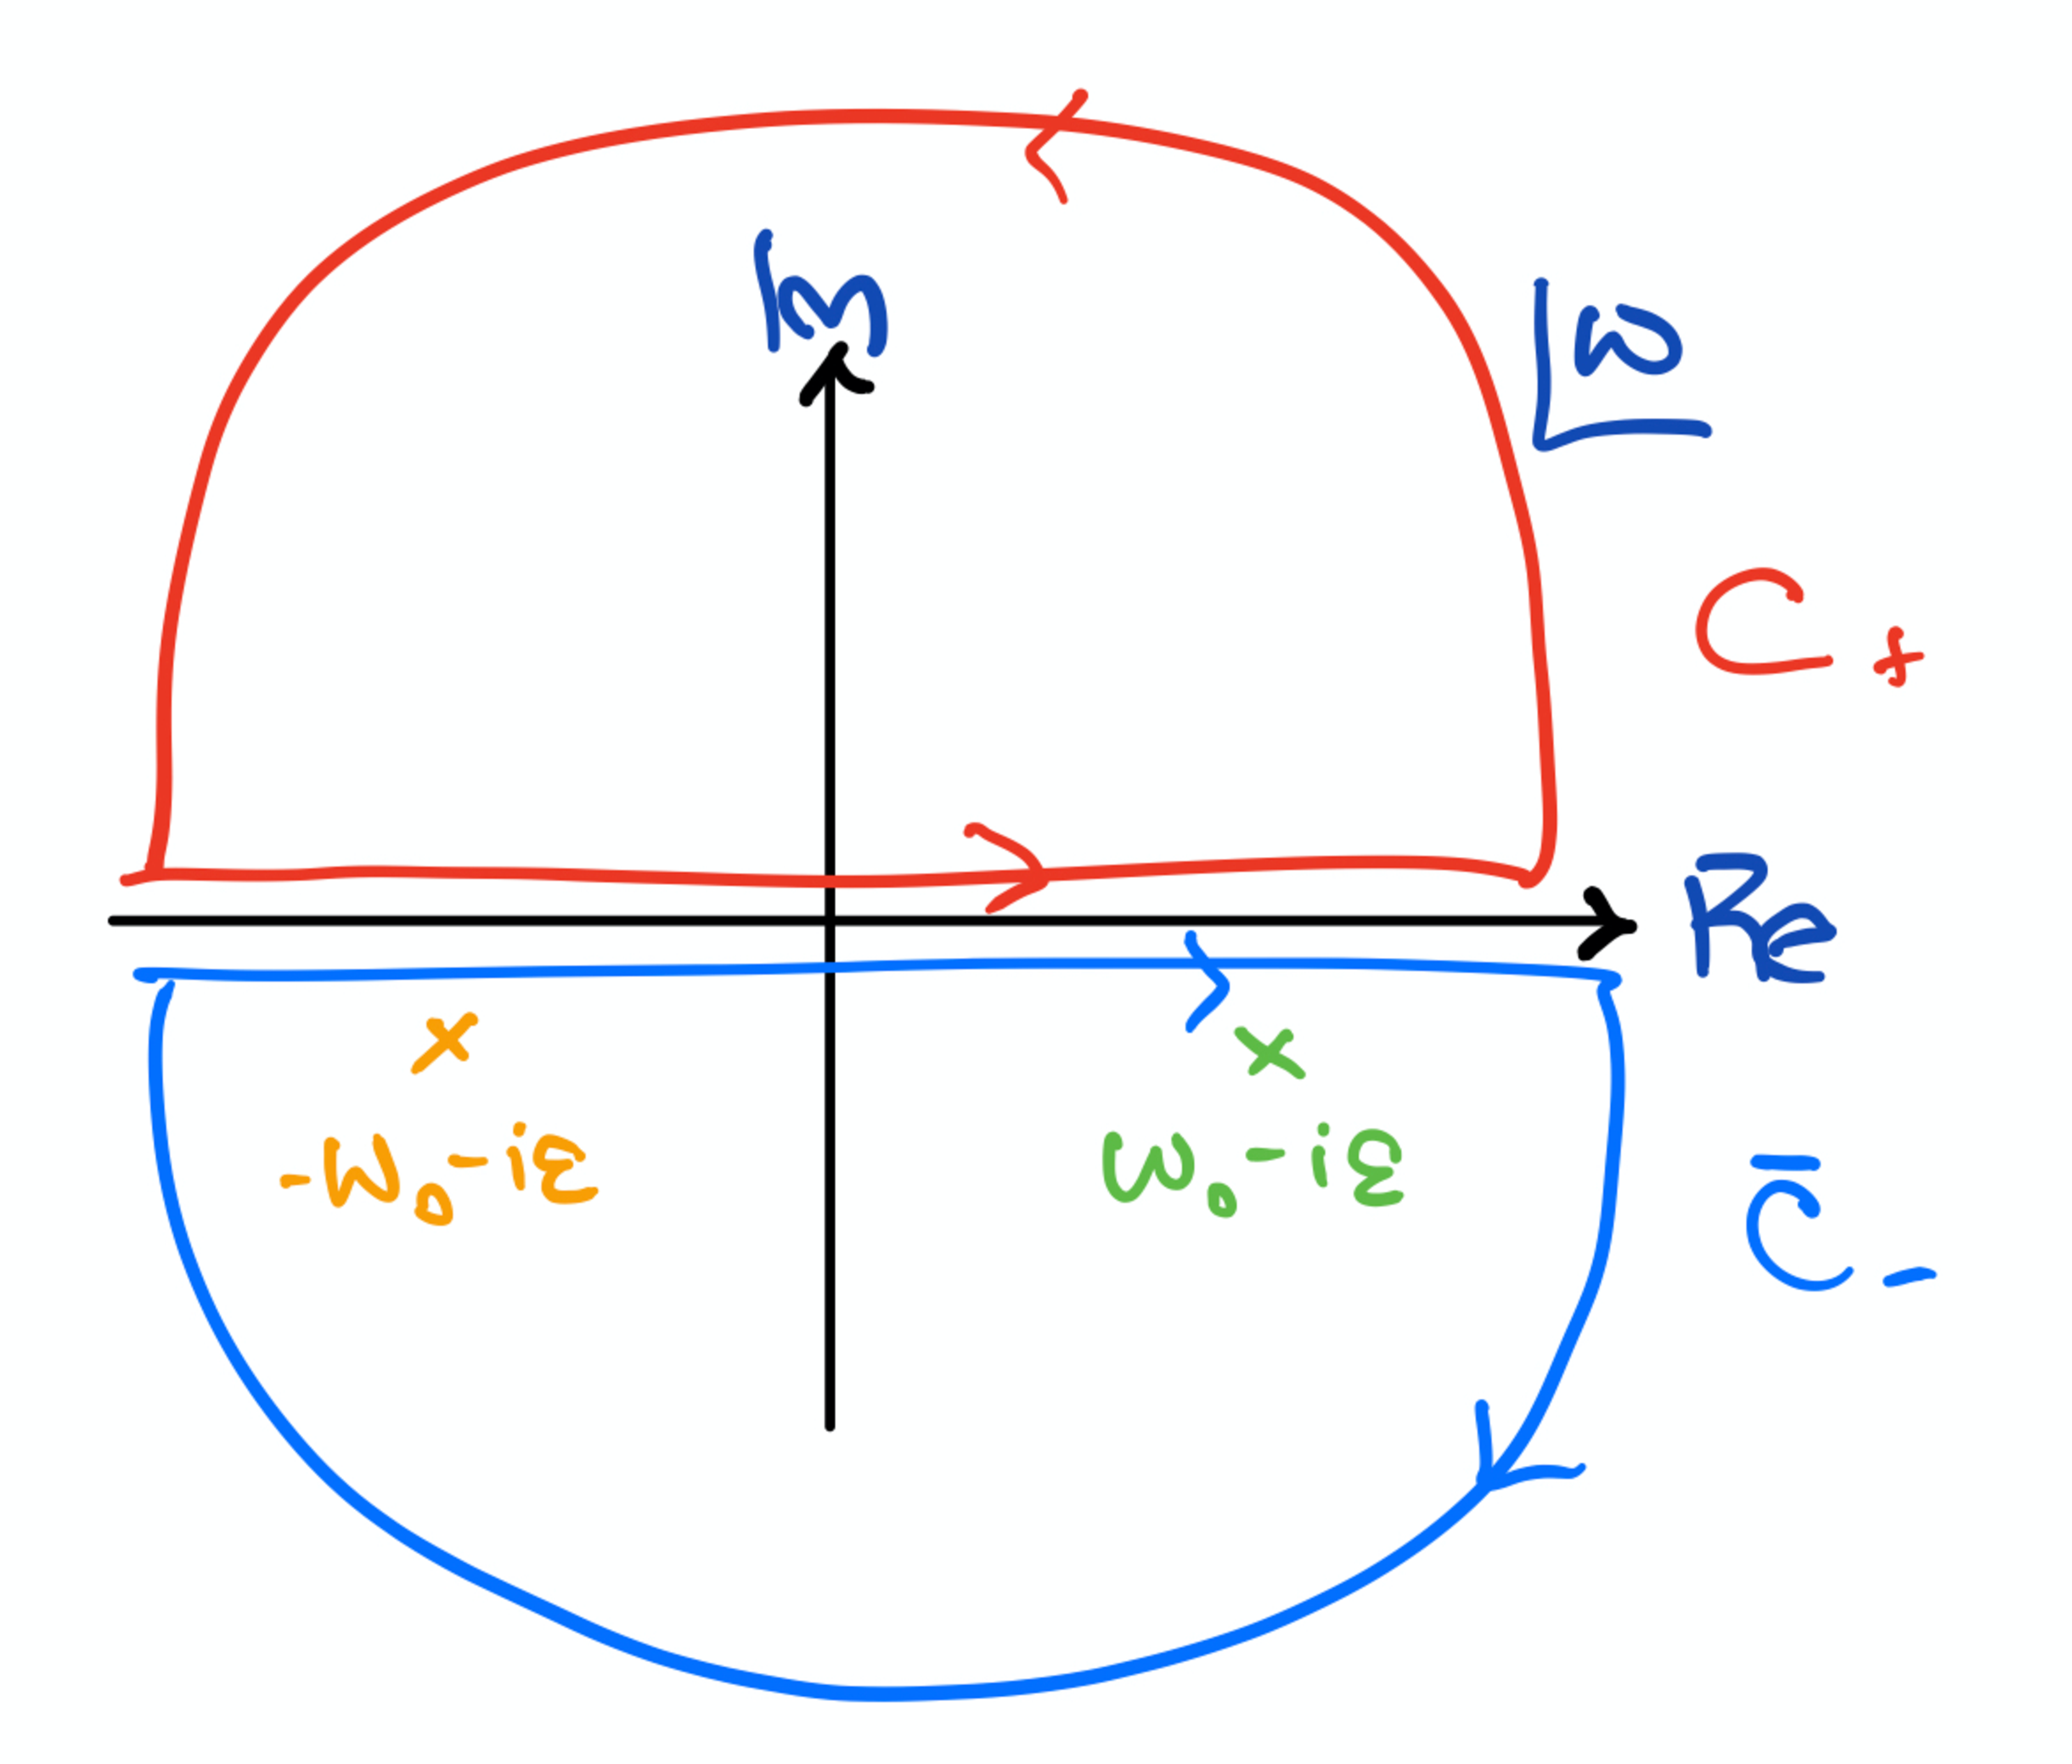
\includegraphics[width=.4\textwidth]{figures/Lec_2017_16_pokedown.pdf}
\end{center}

The integral is exactly the same, except the sign of $\varepsilon$ has changed. 
\begin{exercise}
Pop quiz! Unlike the advanced Green's function where we gave the poles a small positive imaginary part, we have now given the poles a small \textbf{negative} imaginary part. How do we assign the contours $C_+$ and $\bar C_-$ to the cases $t>0$ and $t<0$?
\end{exercise}
Did I fool you? The poles may have moved, but the way that we pick contours does not change: this is fixed by the $e^{-i\omega t}$ factor in the integrand. Thus we \emph{still} have the contour choices in \eqref{eq:t:sign:contour:HO}:
\begin{align}
	t>0 &\to \bar C_{-} 
	&
	t<0 &\to C_+ \ .
\end{align}
What has changed is that now the $\bar C_{-}$ contour encloses poles, whereas the $C_+$ contour encloses no poles. This clearly tells us that the integral over $\omega$ (or its complexificaion $z$) is zero for $t<0$, which means we do not have acausal propagation: 
\begin{align}
	G(t<0) &= 0 \ .
	\label{eq:HO:G:ret:acausal}
\end{align}

What about the causal propagation? Remember that $\bar C_{-}$ has a negative orientation. To keep our signs clear, let's write the integral as negative a contour $C_-$  which has the positive orientation: 
\begin{align}
	\oint_{\bar C_-} = -\oint_{C_-} \ .
\end{align}
We can go ahead and do the integral over $C_-$ using the residue theorem. We're simply re-doing \eqref{eq:HO:G:integral:adv:} and \eqref{eq:HO:G:integral:adv:2} with $\varepsilon\to -\varepsilon$. Writing $f(z)$ to be the integrand, we have:
\begin{align}
	G(t>0) =& 
	-\frac{1}{2\pi} \oint_{C_-}dz\, f(z)
	\\
	=&
	2\pi i \times -\frac{1}{2\pi} 
	\left(\text{Res}_f(\omega_0) + \text{Res}_f(-\omega_0)\right)
	\\
	=& \frac{1}{\omega_0}\sin(\omega_0 t) \ .
\end{align}
Combining this with \eqref{eq:HO:G:ret:acausal} using the Heaviside $\Theta$-function \eqref{eq:Heaviside:Theta} gives the \textbf{retarded Green's function}:
\begin{align}
	G_\text{ret}(t) &= 
	\frac{1}{\omega_0}
	\sin(\omega_0 t)
	\Theta(t) \ .
\end{align}
\begin{exercise}
Restore $t_0\neq$ in the above equation for the retarded Green's function.
\end{exercise}
By the way, we will often use the word \textbf{propagator} in place of Green's function. This is because the Green's function propagates information from the source to the observation point\footnote{This is especially clear when solving linear differential equations for which the Green's function represents an exact solution. For non-linear problems, one typically resorts to a perturbation expansion. This is what Feynman diagrams are: lines represent propagators, which are Green's functions for the linear part of the dynamical equation. The vertices represent non-linearities which must be treated as a Taylor series about a partition function.}. 





